\chapter{Appendix A}
\label{app:app01}

\initial{I}n this appendix we will present all the tests for the 12-year dataset, which have already been performed and explained in Chapter \ref{chap:NN-model} and Chapter \ref{chap:results} for the 6-year dataset. 
We begin by presenting the histograms for several flux bins (Fig. \ref{fig:12y-hist}). As we can see, the histograms are properly centered apart from the case of really high flux and extremely low flux, which means that the prediction of the neural network for the $dN/dS$ might not be perfectly accurate over $S=3\cdot 10^{-8} $cm$^{-2}$s$^{-1}$ and under $S=2 \cdot 10^{-11} $cm$^{-2}$s$^{-1}$. 
\begin{figure}[t]
\centering
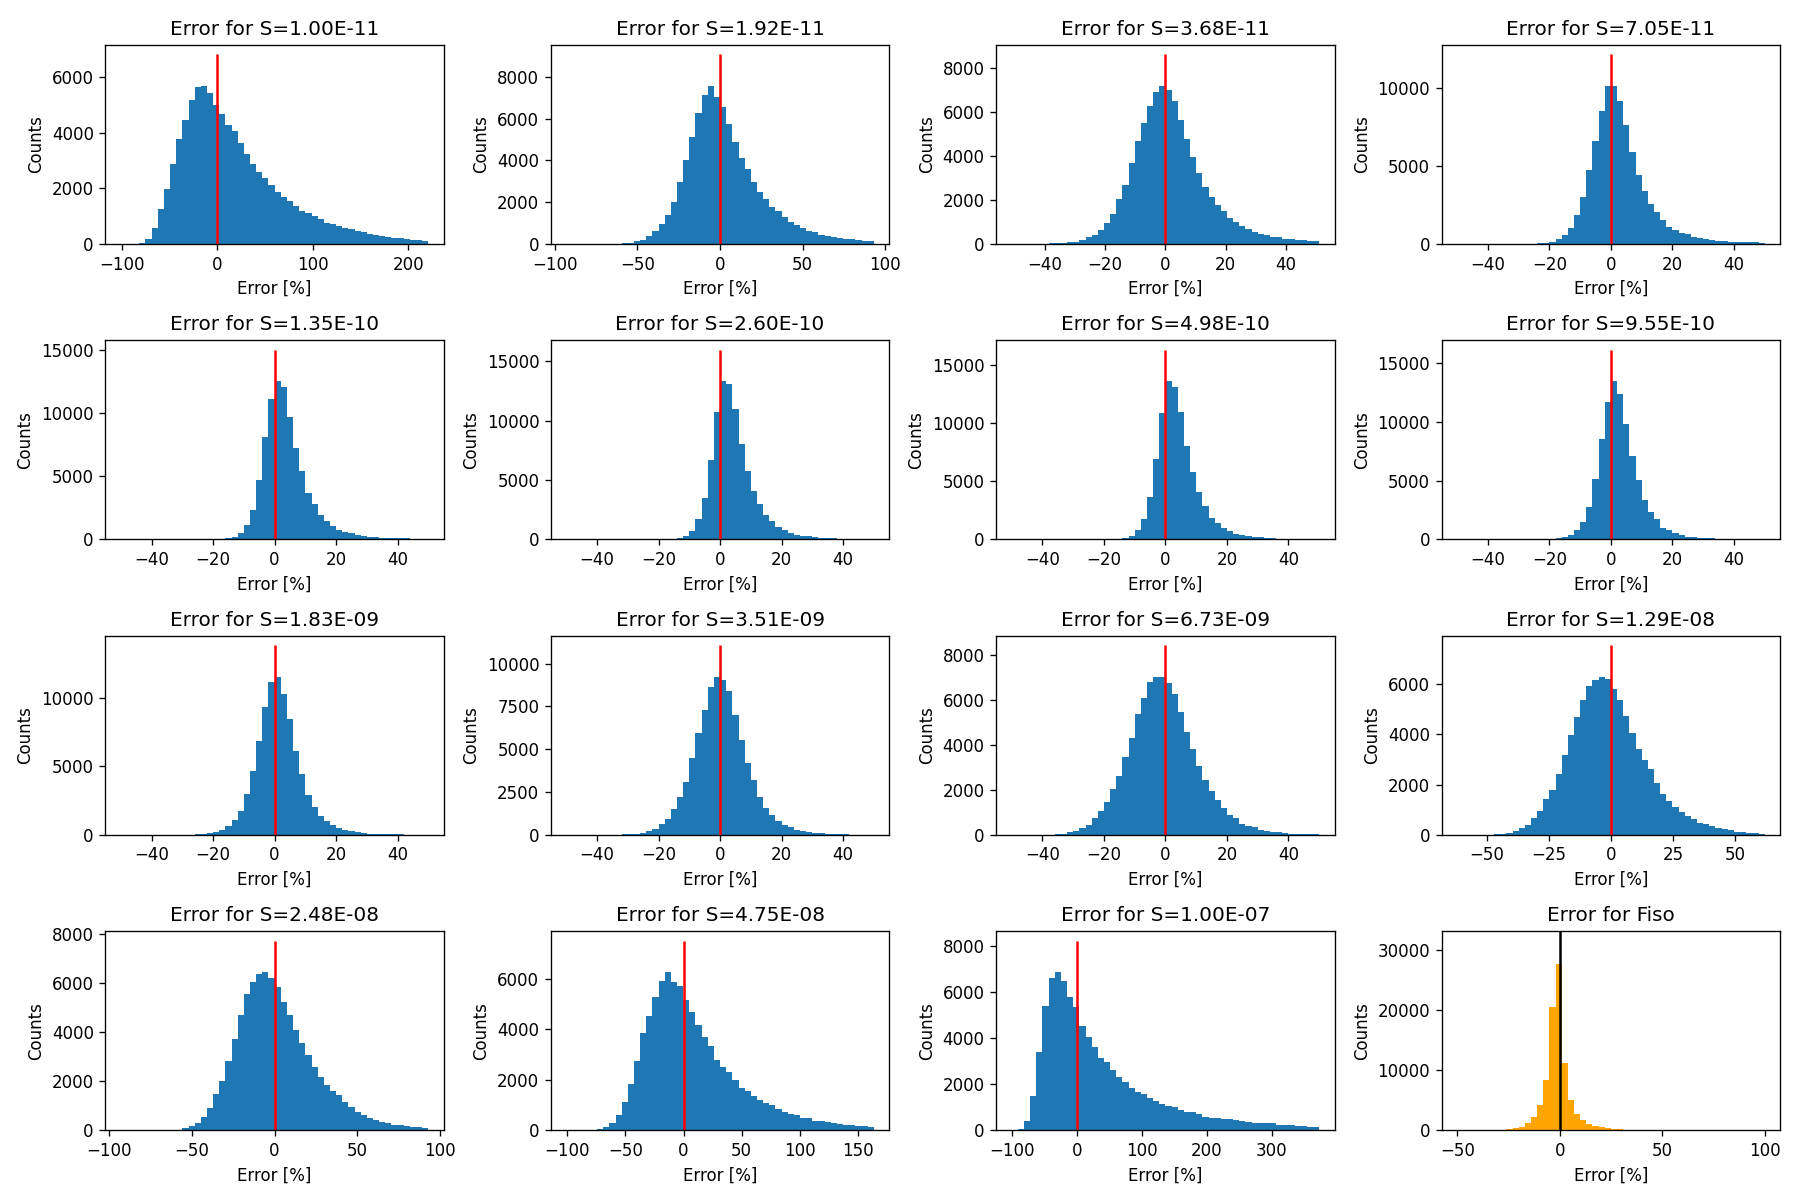
\includegraphics[width=1.0\textwidth]{appendix_A/img/error_histogram.png}
\caption{Error histograms for several flux bins and for $F_{iso}$ for the 12-year dataset.}
\label{fig:12y-hist}
\end{figure}
\noindent
\\
The histogram for the error on the predicted gamma-ray flux is shown in Fig. \ref{fig:12y-flux-hist}. As we can see, it is well centered and the $1\sigma$ band is (-3.4\%, 2.3\%). 

\begin{figure}[t]
\centering
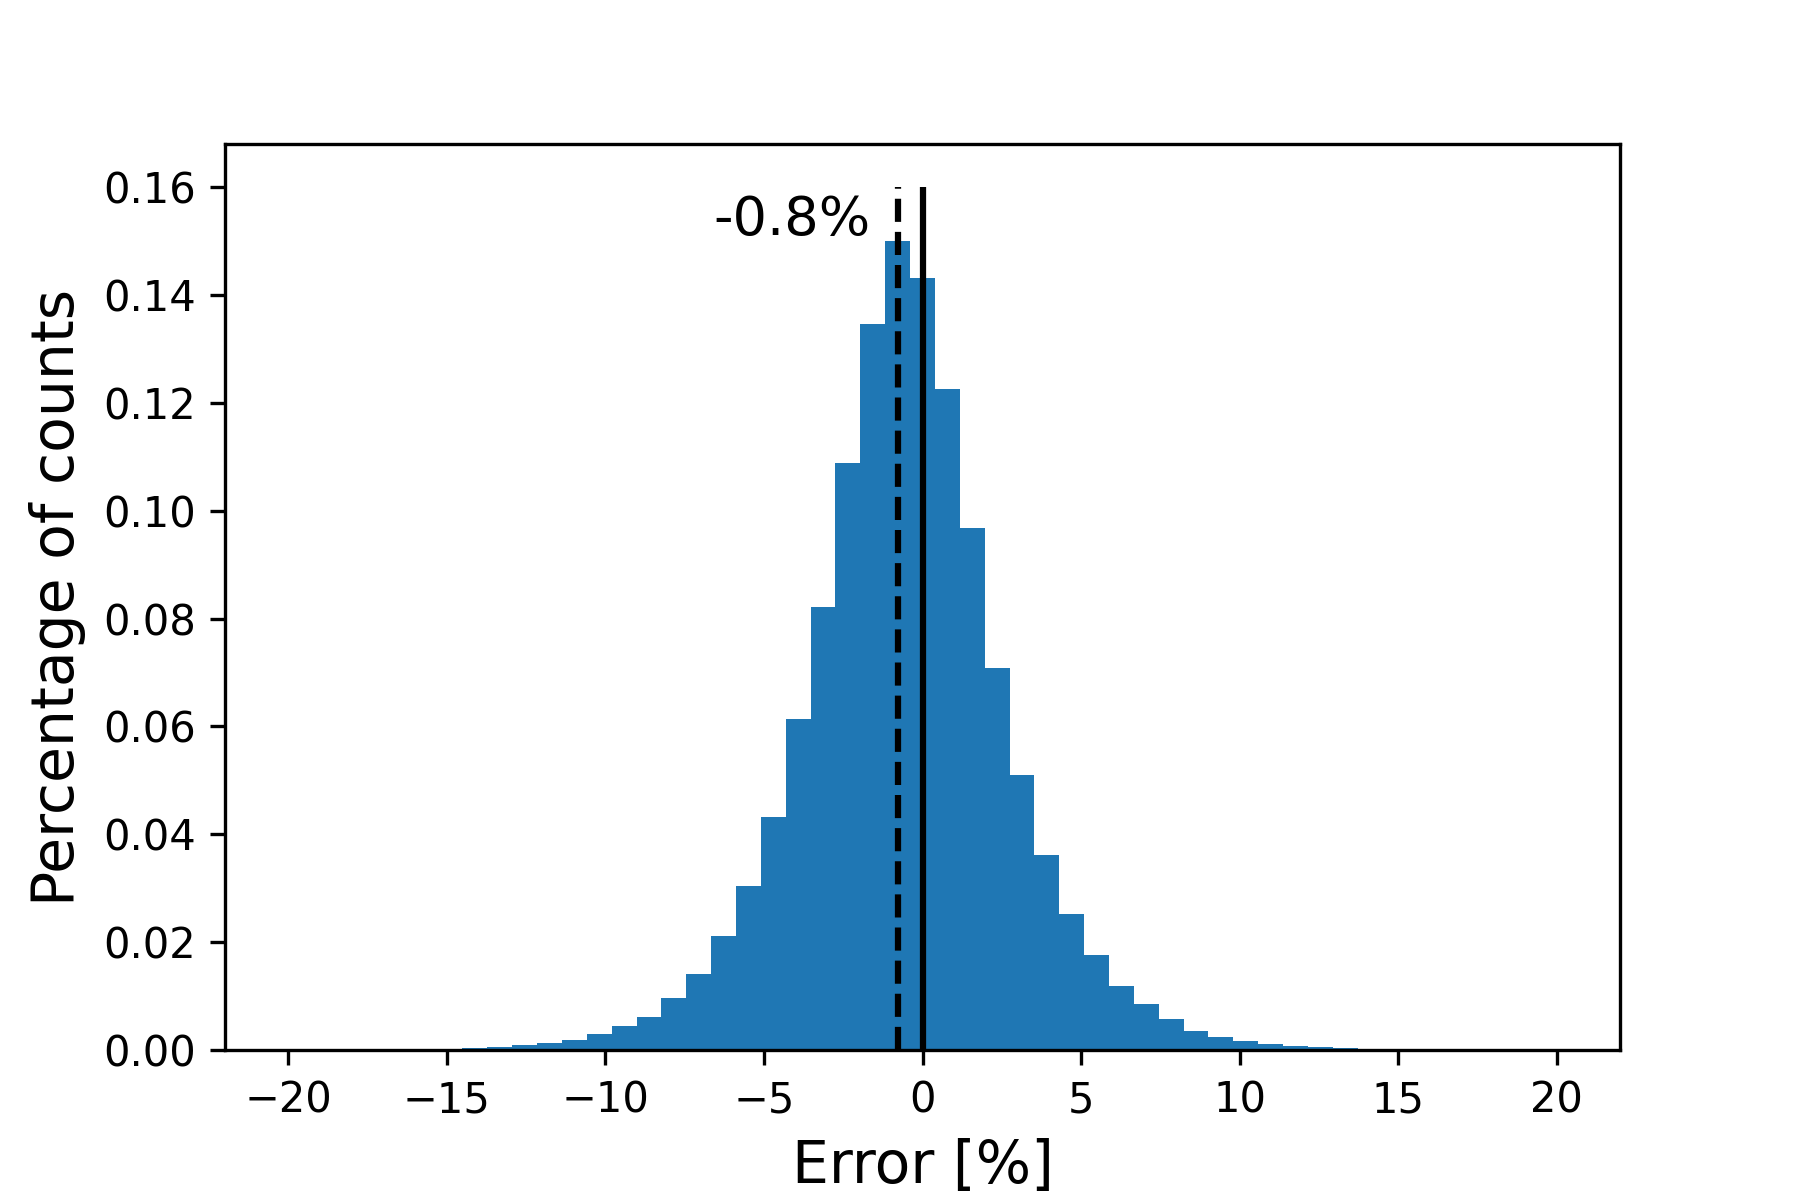
\includegraphics[width=0.7\textwidth]{appendix_A/img/total_flux_hist_with_map.png}
\caption{Error histogram for the predicted gamma-ray flux for the 12-year dataset.}
\label{fig:12y-flux-hist}
\end{figure}
\noindent
\\
After estimating the error bands, we have studied the prediction from random test maps (Fig. \ref{fig:12y-random}). In general, the neural network reconstructs properly the original $dN/dS$, regardless of the high noise introduced by $F_{iso}=4\cdot 10^{-7} $cm$^{-2}$s$^{-1}$sr$^{-1}$.
\begin{figure}[t]
\centering
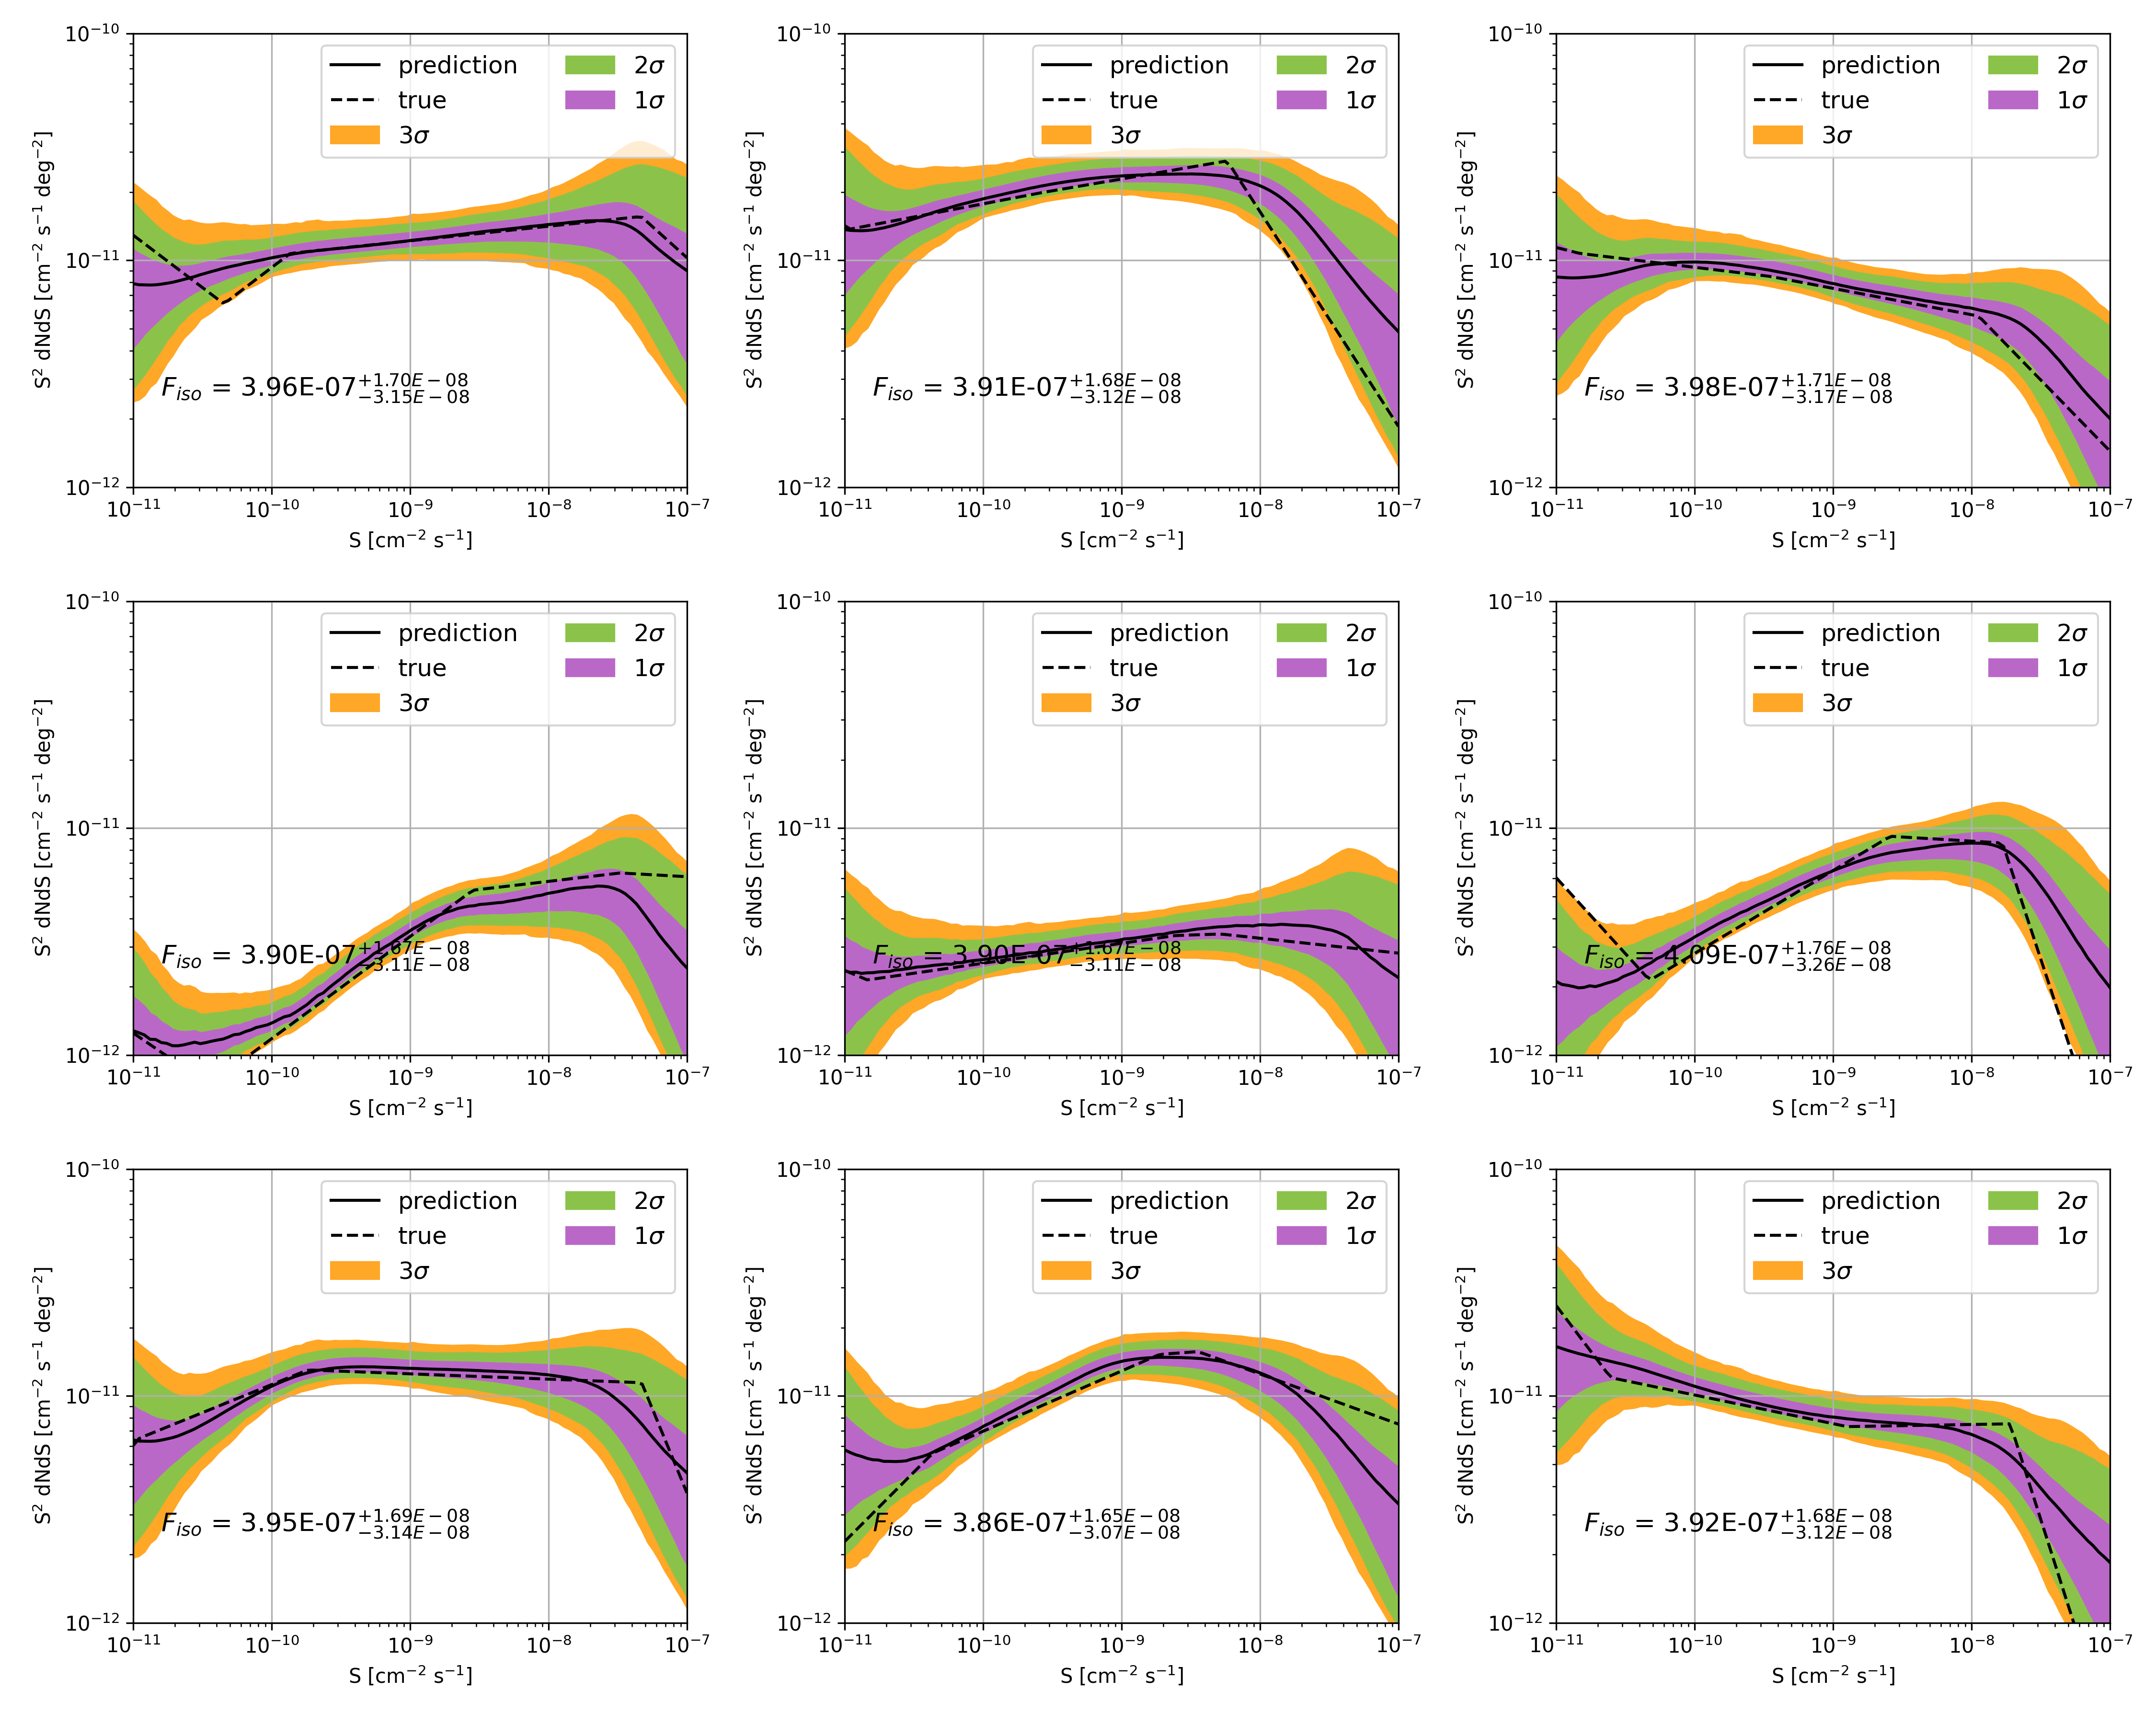
\includegraphics[width=1\textwidth]{appendix_A/img/random_maps.png}
\caption{Prediction for several random maps, with reference $F_{iso}=4\cdot 10^{-7} $cm$^{-2}$s$^{-1}$sr$^{-1}$), and with sources from  $S=10^{-11}$cm$^{-2}$s$^{-1}$, 12-year dataset.}
\label{fig:12y-random}
\end{figure}
\noindent
\\
We have then performed the tests with $dN/dS$ functions of fixed slope (Section \ref{sec:fixed-slope}), which are represented in Fig. \ref{fig:12y-slope}. As we can see, the neural network performs arguably well in the whole flux range. 
\begin{figure}[t]
\centering
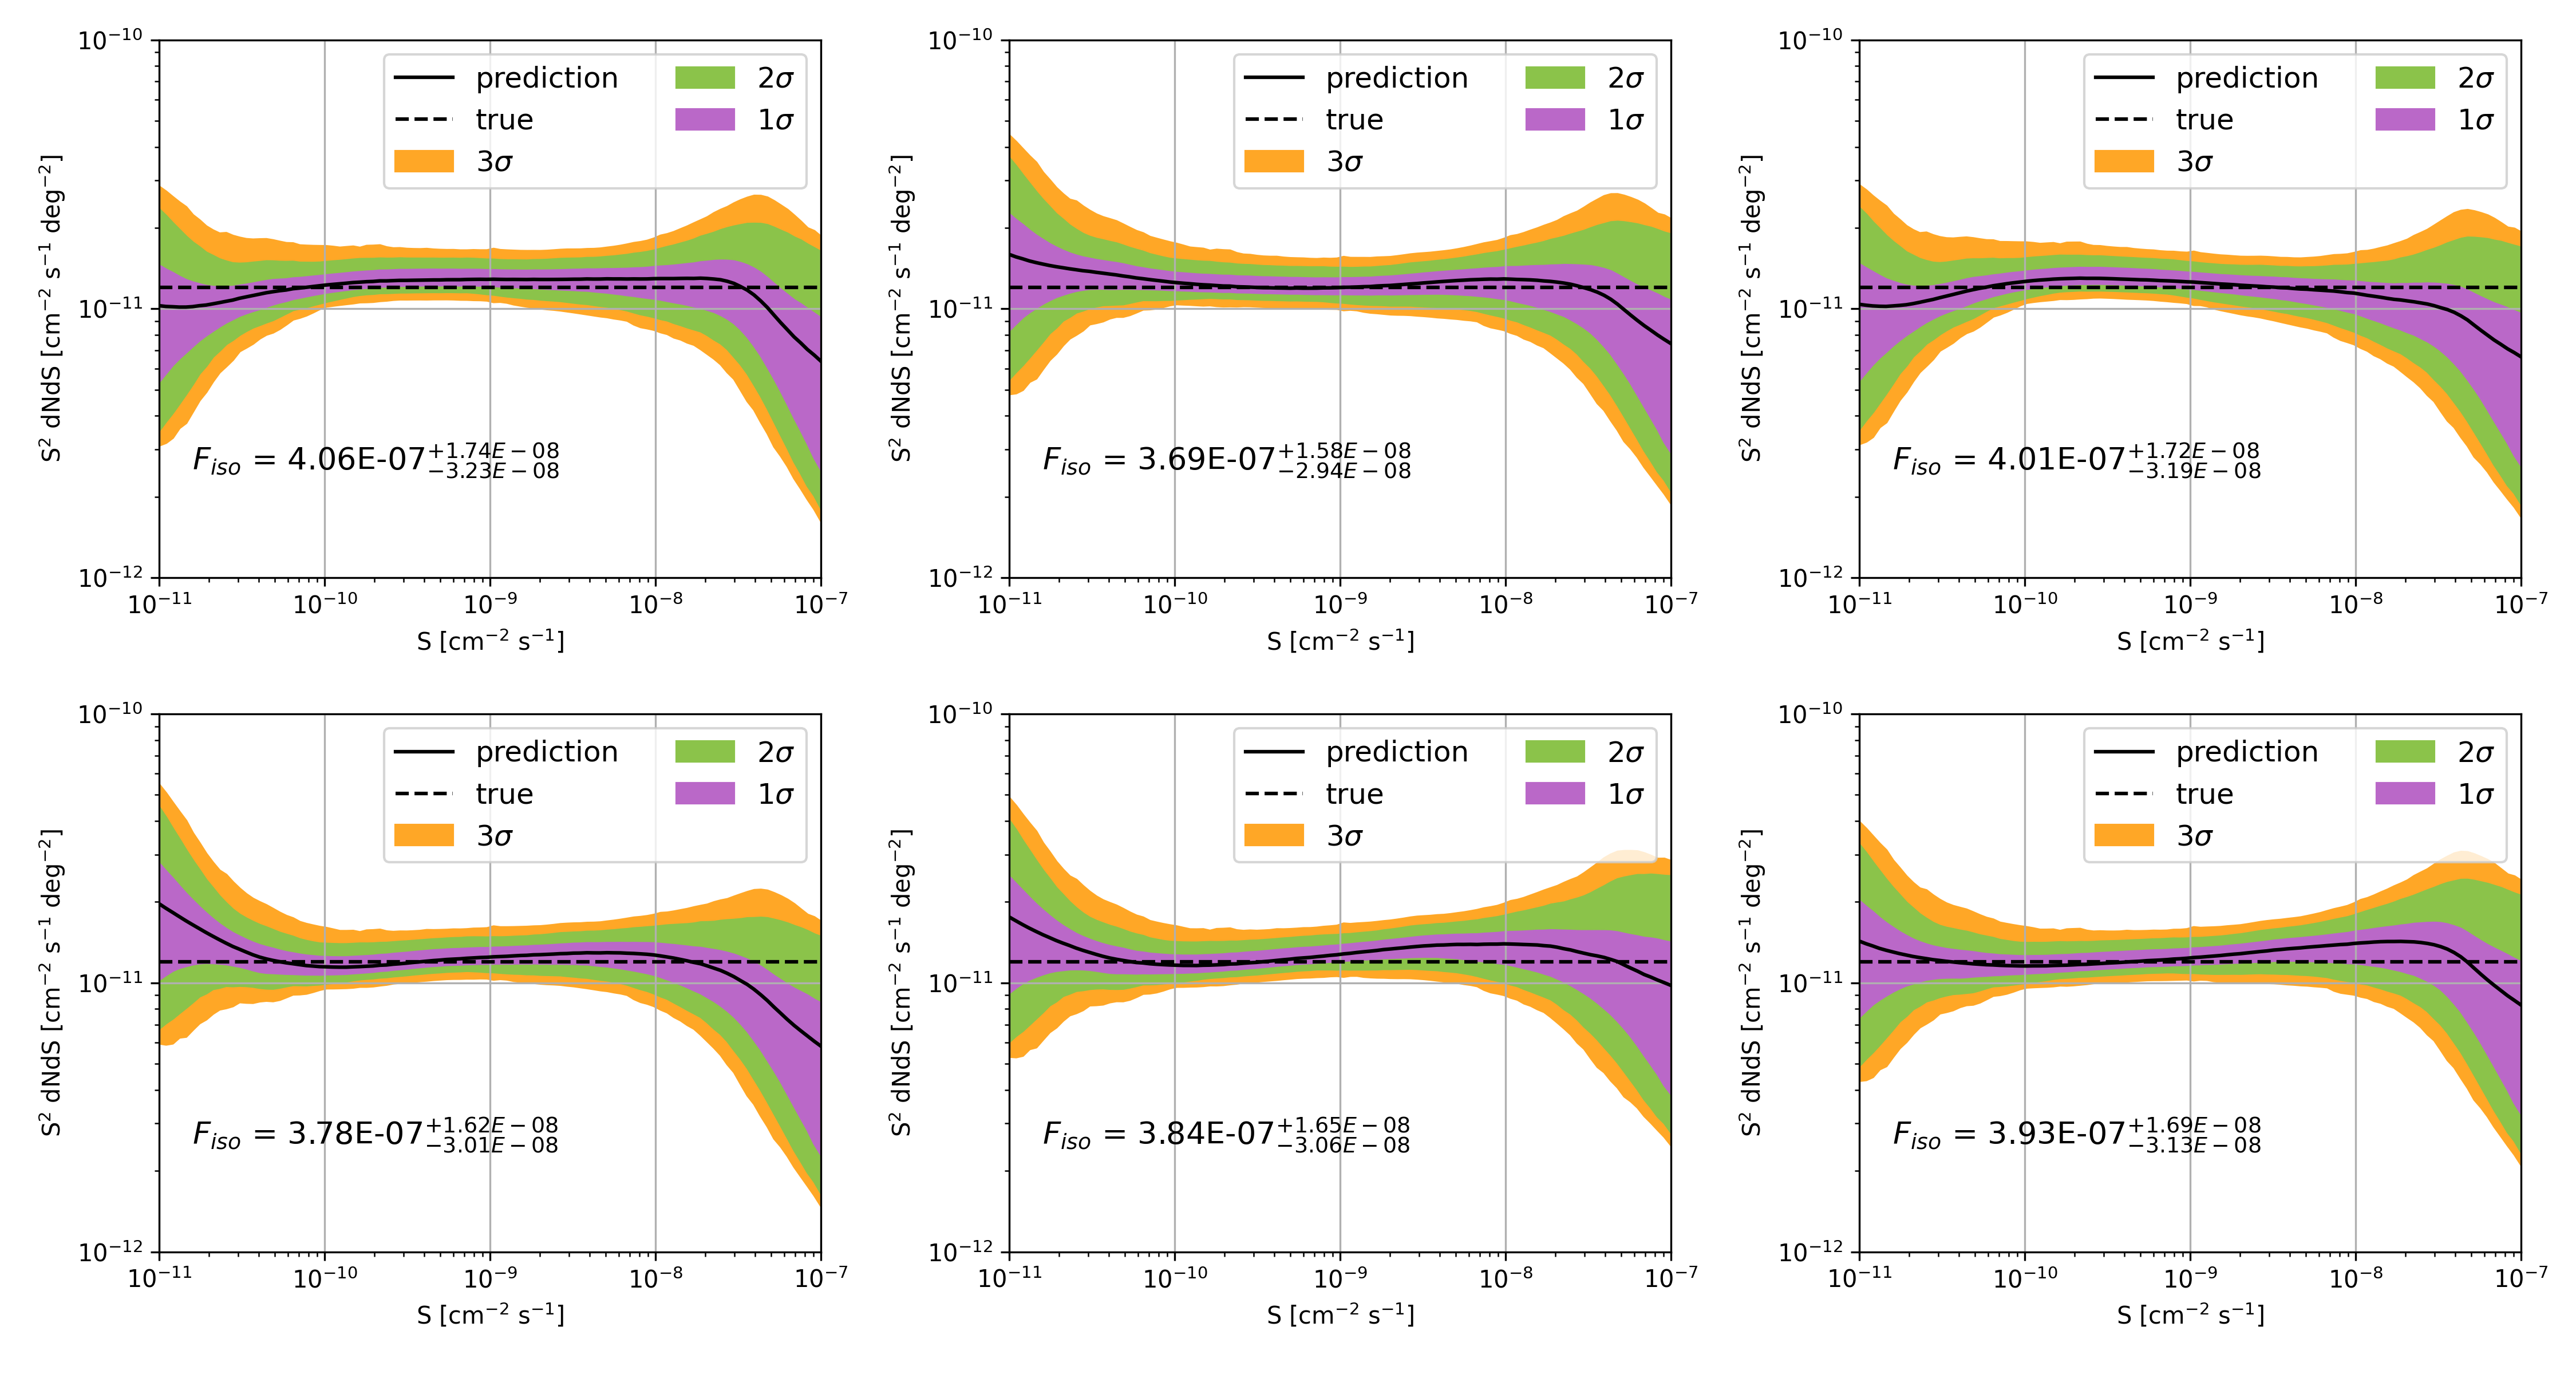
\includegraphics[height=0.3\textheight]{appendix_A/img/pendenza2.png}
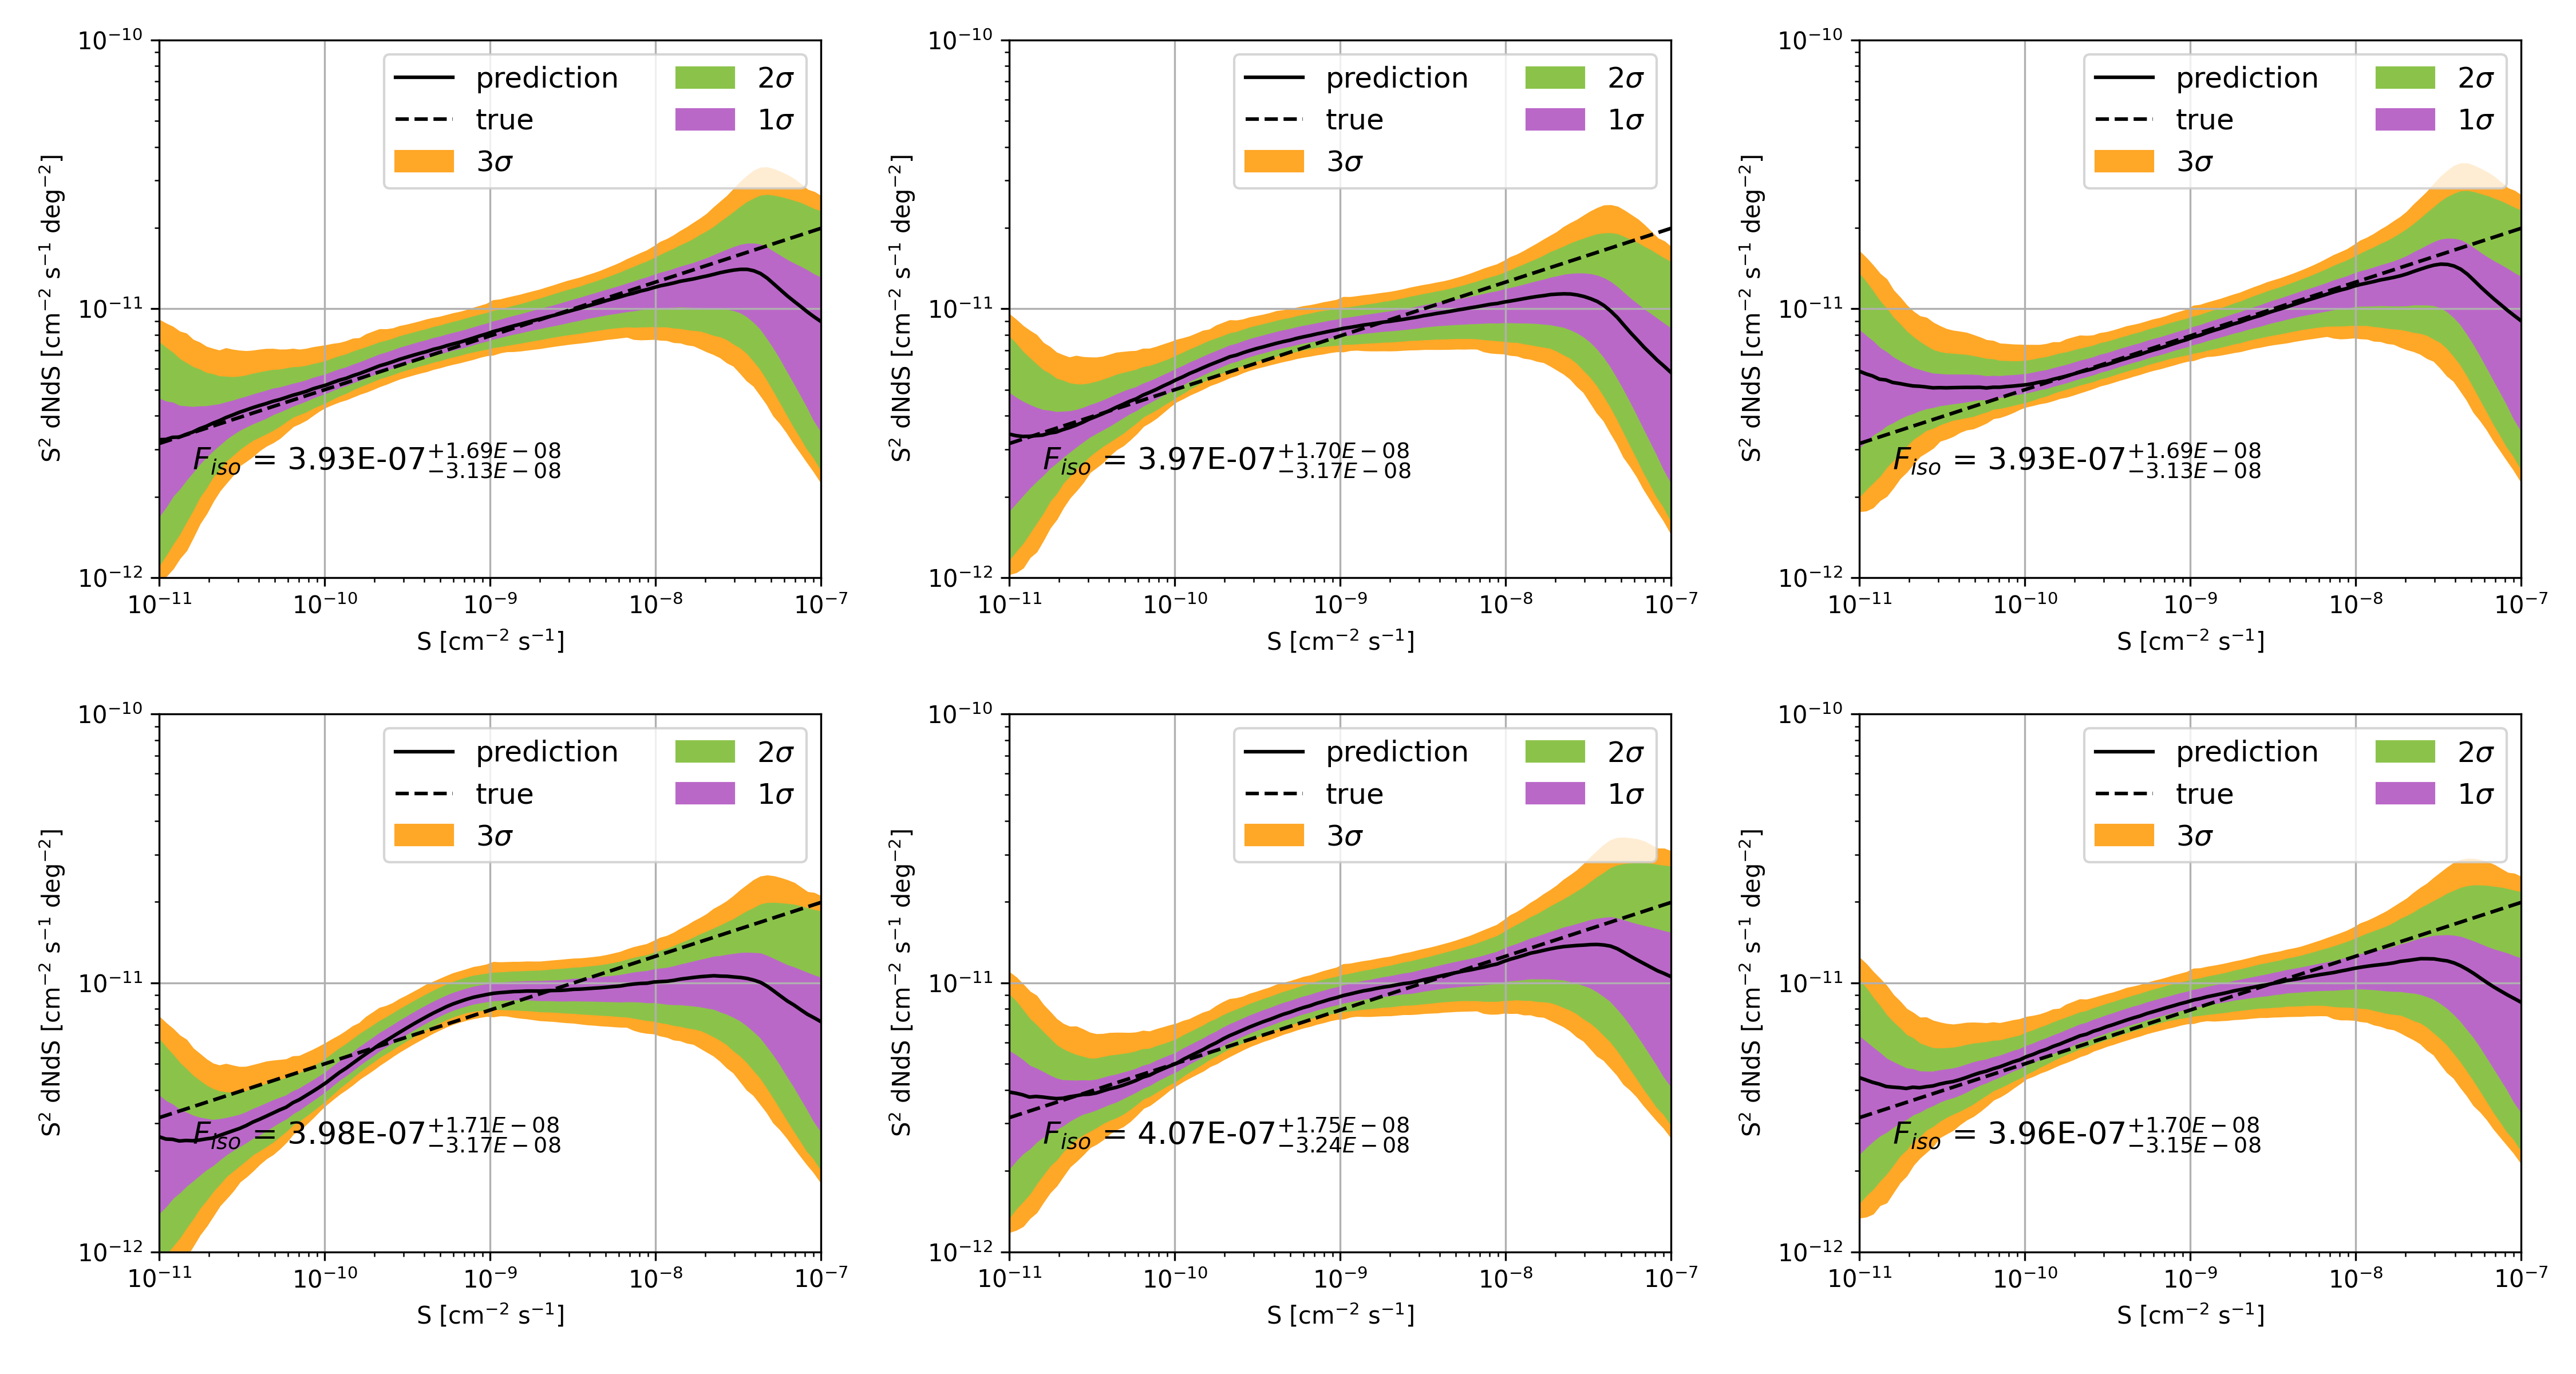
\includegraphics[height=0.3\textheight]{appendix_A/img/pendenza1.8.png}
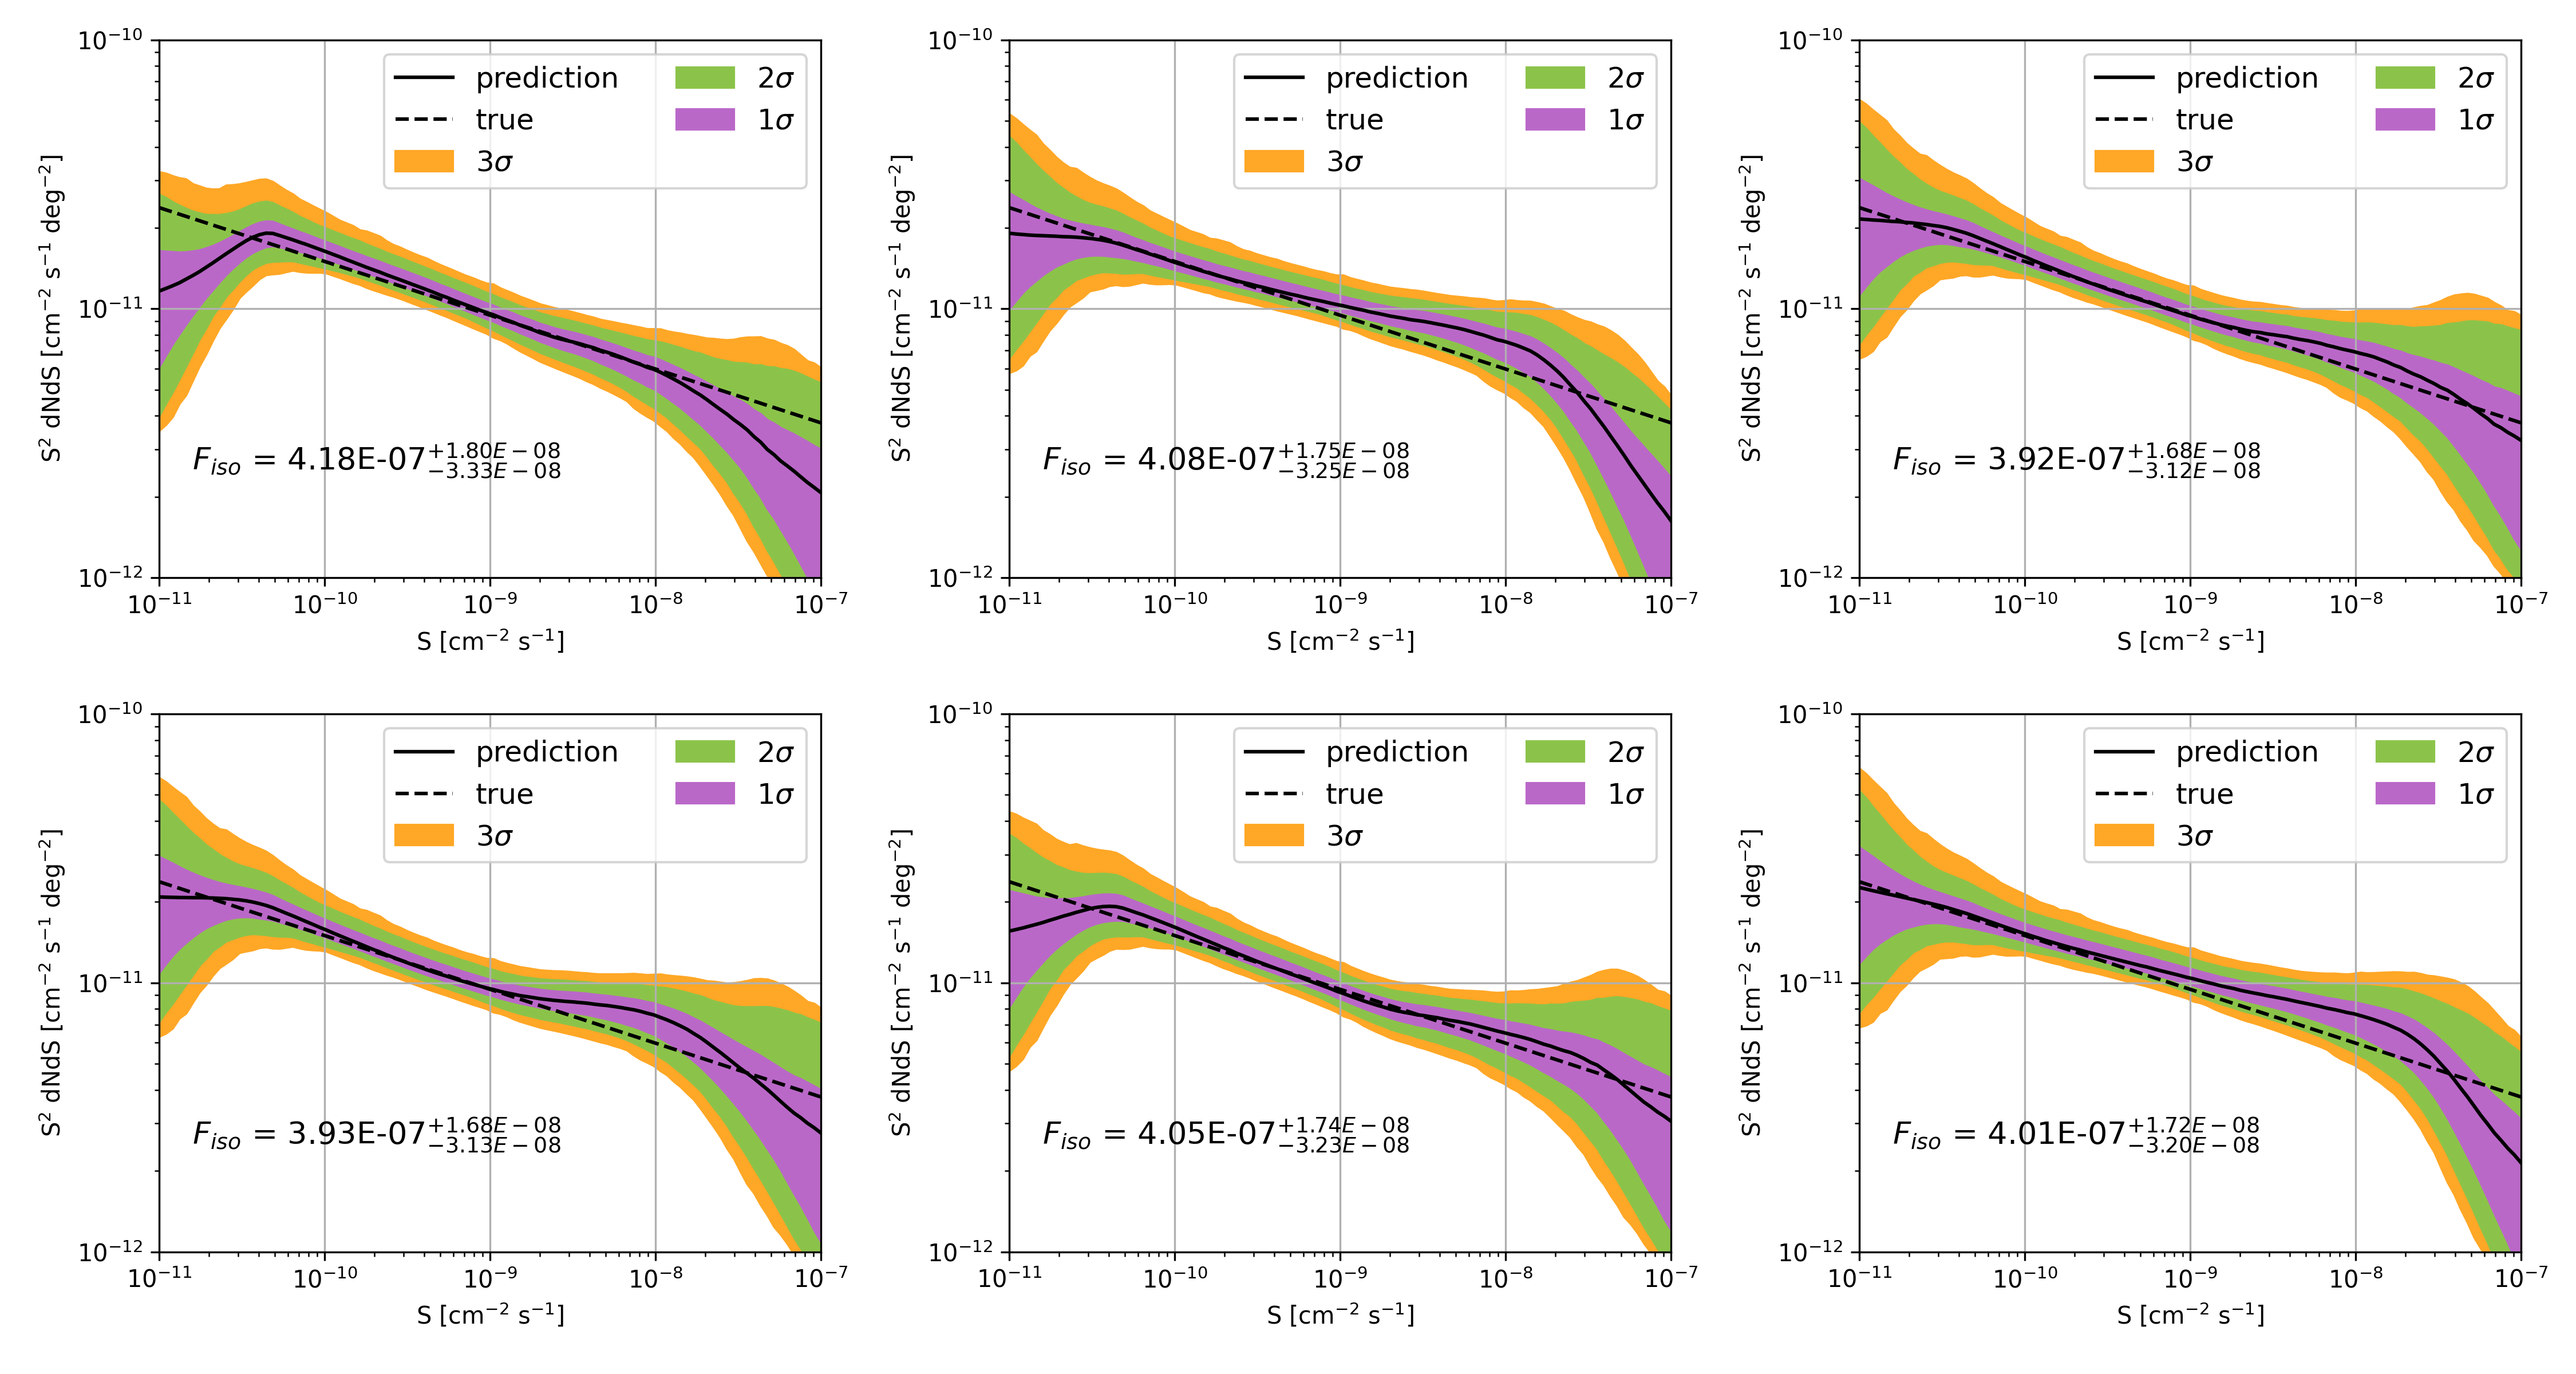
\includegraphics[height=0.3\textheight]{appendix_A/img/pendenza2.2.png}
\caption{Prediction for several maps of fixed slope, with reference $F_{iso}=4\cdot 10^{-7} $cm$^{-2}$s$^{-1}$sr$^{-1}$, and with sources from  $S=10^{-11}$cm$^{-2}$s$^{-1}$, 12-year dataset. {\em Top:} $dN/dS \sim S^{-2}$. {\em Middle:} $dN/dS \sim S^{-1.8}$. {\em Bottom:} $dN/dS \sim S^{-2.2}$.}
\label{fig:12y-slope}
\end{figure}
\noindent
\\
As a last test, we have then performed the procedure described in Section \ref{sec:multipole-subtraction} to remove the residuals of the galactic foreground subtraction up to $\ell_{max}$. It is possible to find the results of this analysis in Fig. \ref{fig:12y-mappe-ripulite}. Similar considerations to the ones for the 6-year case still hold, and we do not experience significative changes or improvements. 
\begin{figure}[t]
\centering
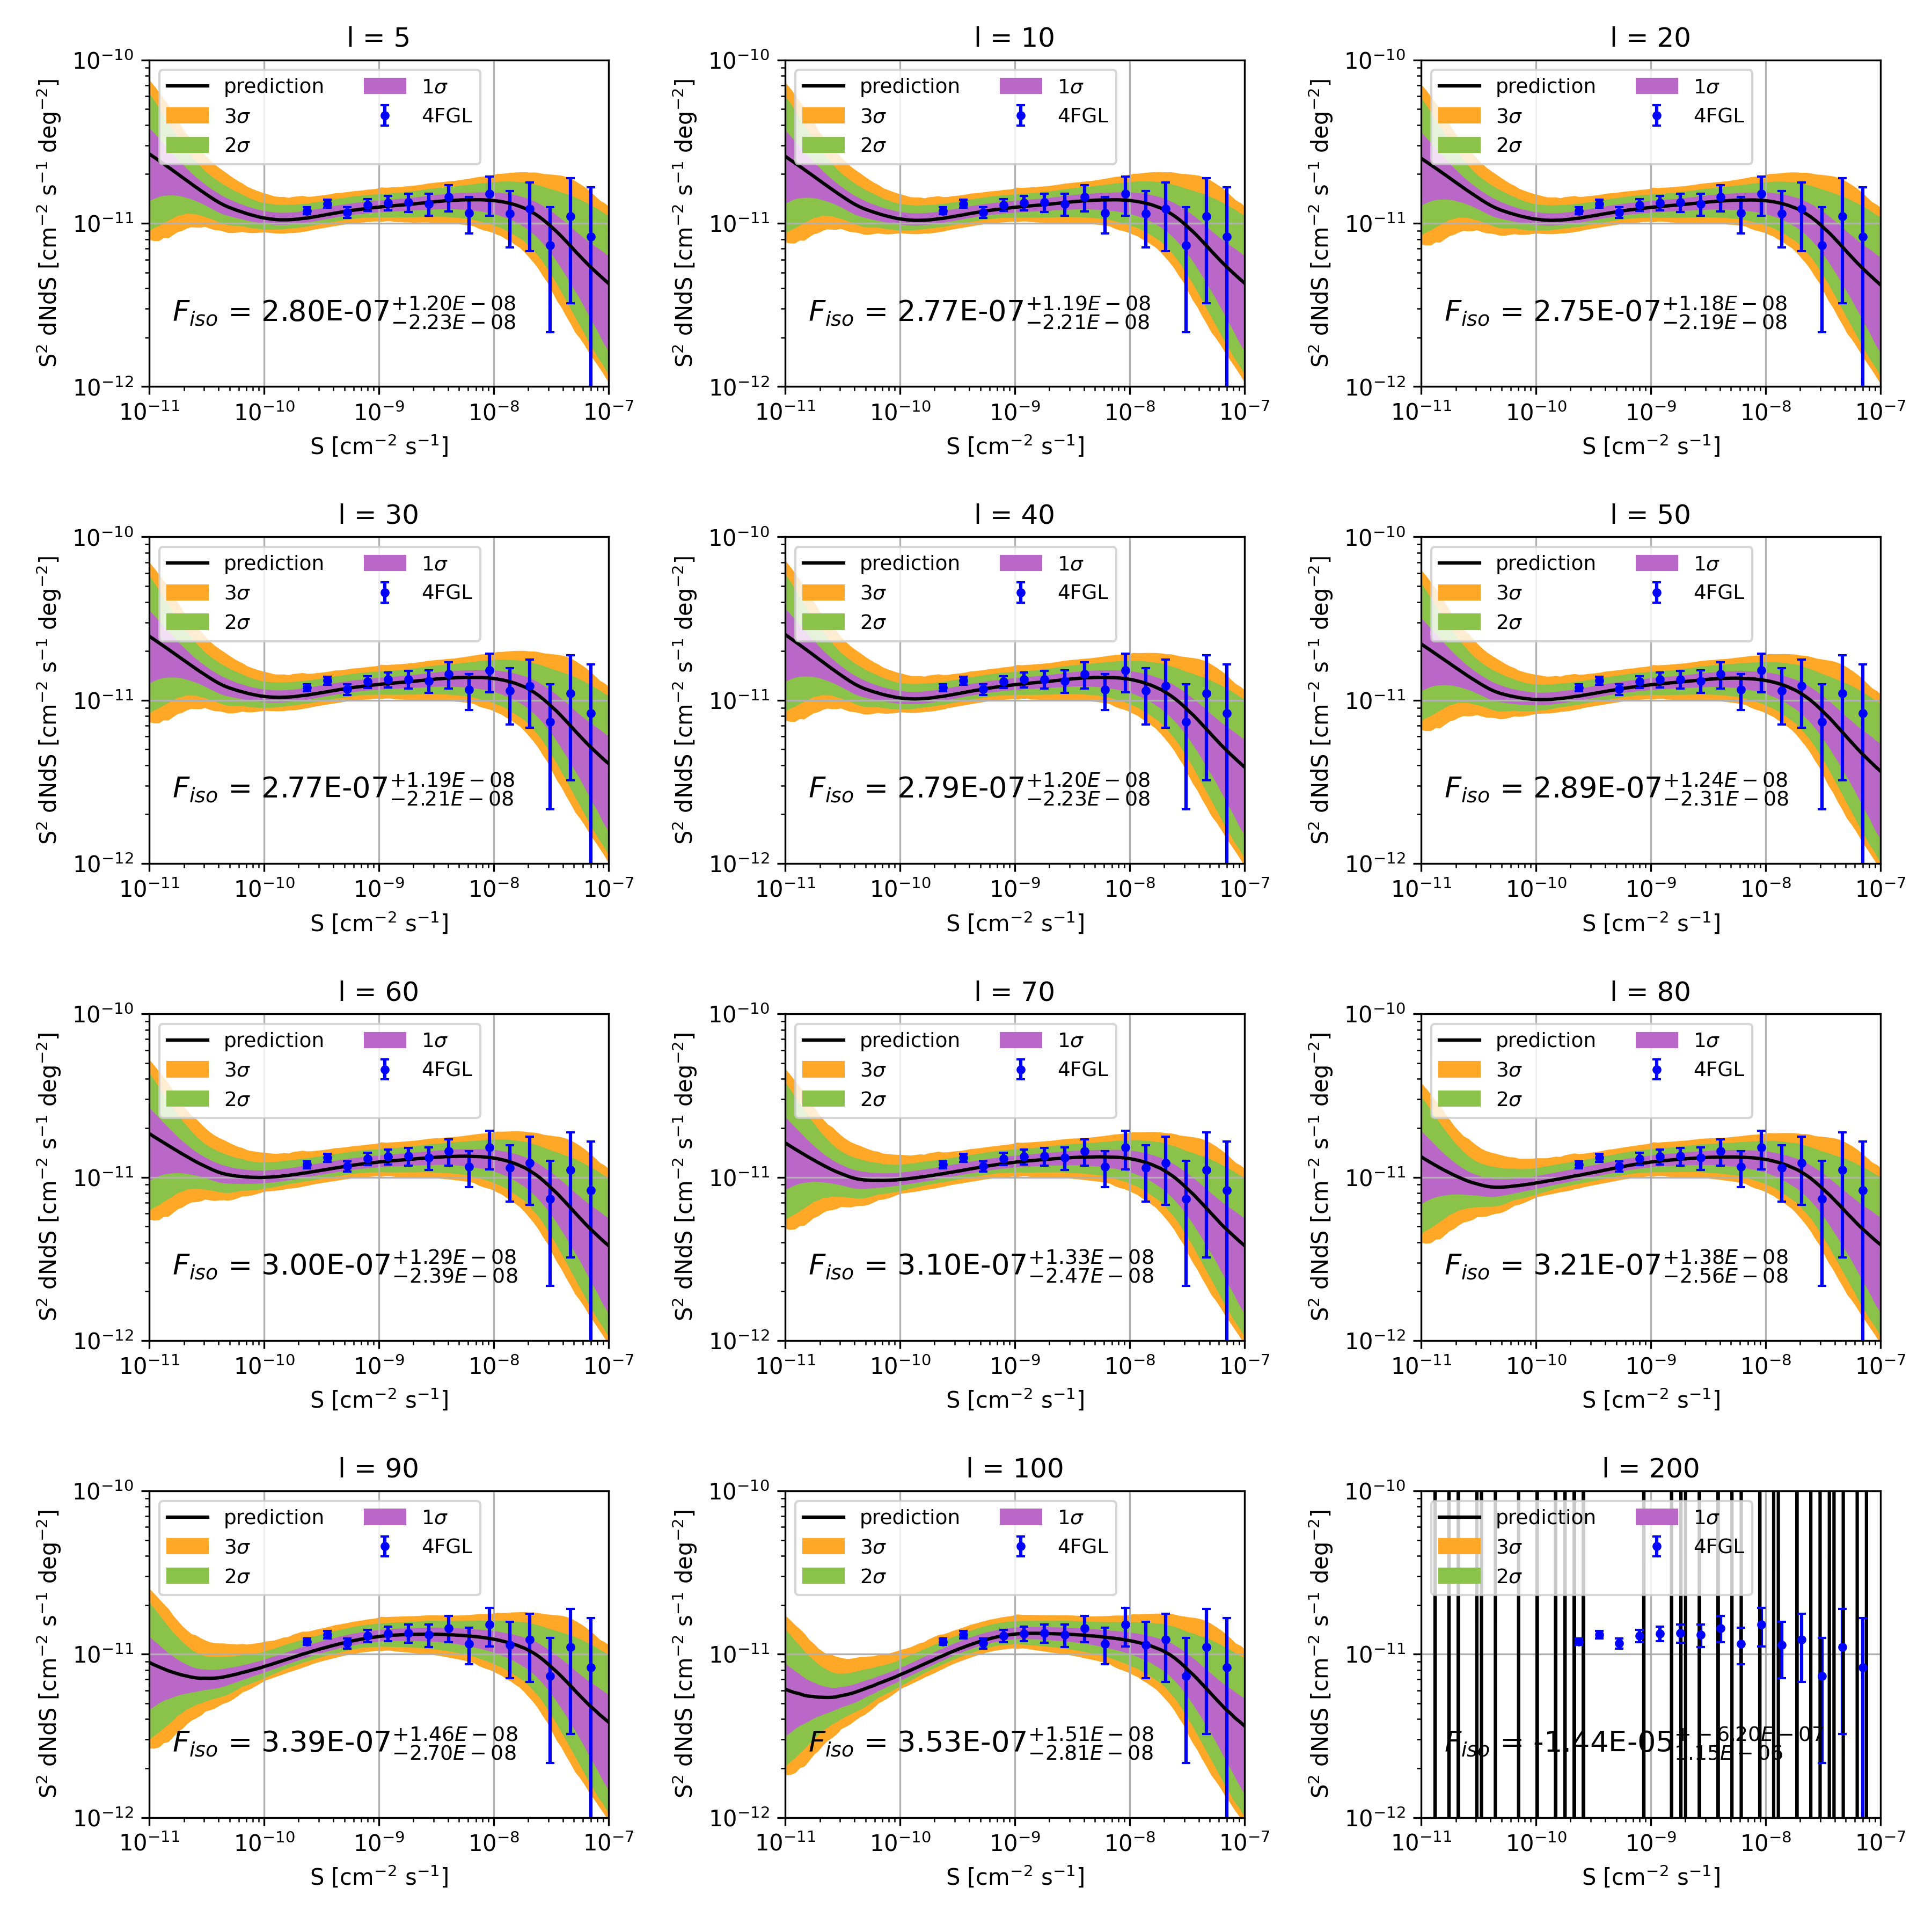
\includegraphics[width=1\textwidth]{appendix_A/img/mappe_ripulite.png}
\caption{Test predictions for Fermi photon counts maps whose galactic foreground subtraction has been improved through the artificial removal of residual components up to a multipole $\ell_{max}$. 12-year dataset.}
\label{fig:12y-mappe-ripulite}
\end{figure}
\noindent